\documentclass[12pt]{article}
\usepackage[utf8]{inputenc}
\usepackage{graphicx} % Allows you to insert figures
\usepackage{amsmath} % Allows you to do equations
\usepackage{fancyhdr} % Formats the header
\usepackage{geometry} % Formats the paper size, orientation, and margins
\usepackage[style=authoryear-ibid,backend=biber]{biblatex} % Allows you to do citations - does Harvard style and compatible with Zotero

% PARA IMAGNES E SUBIMAGENS
\usepackage{graphicx}
\usepackage{subcaption}
\usepackage{mwe}

\usepackage[section]{placeins}
\usepackage{hyperref}
\usepackage{listings}

\usepackage{amsmath}

\addbibresource{Example.bib} % Tells LaTeX where the citations are coming from. This is imported from Zotero
\usepackage[english]{babel}
\usepackage{csquotes}
\renewcommand*{\nameyeardelim}{\addcomma\space} % Adds comma in in-text citations
\linespread{1.25} % About 1.5 spacing in Word
\setlength{\parindent}{0pt} % No paragraph indents
\setlength{\parskip}{1em} % Paragraphs separated by one line
\renewcommand{\headrulewidth}{0pt} % Removes line in header
\geometry{legalpaper, portrait, margin=1in}
\setlength{\headheight}{14.49998pt}

\begin{document}
\begin{titlepage}
   \begin{center}
        \vspace*{5cm}

        \Huge{Lesson 1 - three.js Introduction}

        \vspace{0.5cm}
        \LARGE{} % Optional Subtitle Below
            
        \vspace{3 cm}
        \Large{Course: Information Visualization - 44156}
       
        \vspace{0.25cm}
        \large{André Fernandes (97977) 50.0\%, Gonçalo Machado (98359) 50.0\%}
       
        \vspace{3 cm}
        \Large{11/12/2023}
        
        \vspace{0.25 cm}
        \Large{Class - TP2}
        
        \vspace{5cm}
        \Large{Developed \emph{software} can be found \textbf{\href{https://github.com/goncalo-machado/VI}{here}}.}
       

       \vfill
    \end{center}
\end{titlepage}

\setcounter{page}{2}
\pagestyle{fancy}
\fancyhf{}
\rhead{\thepage}
\lhead{Lesson 1 - three.js Introduction - André and Gonçalo - VI}

% -> Para fazer citações usamos: \autocite{}
%%%%%%%%%%%%%%%%%%%%%%%%%%%%%%%%%%%%%%%%%%%%%%%%%%%%%%%%%%
\section*{Introduction}
\label{intro}

Three.js, a powerful JavaScript library for creating 3D graphics on the web in the Computer Graphics area. In this report, we will delve into the essential aspects of configuring environments and developing visualization pipelines using Three.js. The primary focus areas covered in this report include the configuration of environment, one first example, 2D primitives, addition of color, view-port update and other primitives.

%%%%%%%%%%%%%%%%%%%%%%%%%%%%%%%%%%%%%%%%%%%%%%%%%%%%%%%%%%
\section*{1.1 - three.js configuration}
\label{ex_11}

Three.js is a library built on webGL to abstract some of the difficulties related to low-level graphics and to reduce the quantity of code to produce the visualizations. Its configuration is similar to the one used by webGL. To use three.js, it is necessary to include the lines ilustrated on Figure \ref{figs:htlm_file}.

\begin{figure}[h!]
    \centering
        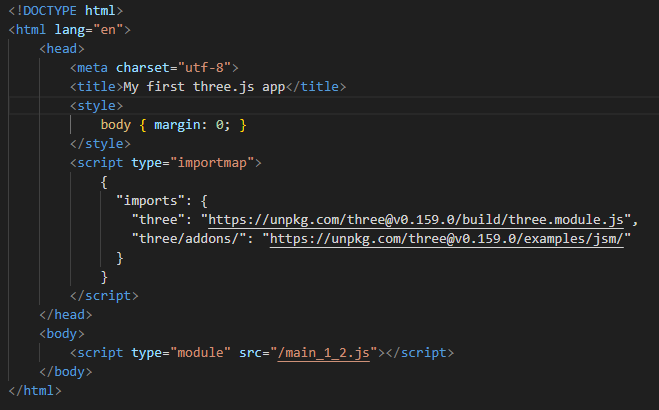
\includegraphics[width = \textwidth]{figs/ex11_1.png}
        \caption{Our html file to run all the java script files.}
        \label{figs:htlm_file}
\end{figure}

In order to make use of the library, it is necessary the following line in each java script file developed:
\begin{lstlisting}

import * as THREE from 'three';

\end{lstlisting}

\pagebreak

%%%%%%%%%%%%%%%%%%%%%%%%%%%%%%%%%%%%%%%%%%%%%%%%%%%%%%%%%%
\section*{1.2 - First example}
\label{sec:ex_12}

For the first example, we had to follow a tutorial available. This tutorial consisted of four steps.\par

The first step consisted in the definition of the scene, camera and renderer, the second in the definition of an object/geometry and camera position, the third in rendering the scene and the fourth one in the scene animation.

%%%%%%%%%%%%%%%%%%%%%%%%%%%%%%%
\subsection{Definition of the scene, camera and renderer}

The code used to make this definitions was the one on Figure \ref{figs:ex12_1}.

\begin{figure}[h!]
    \centering
        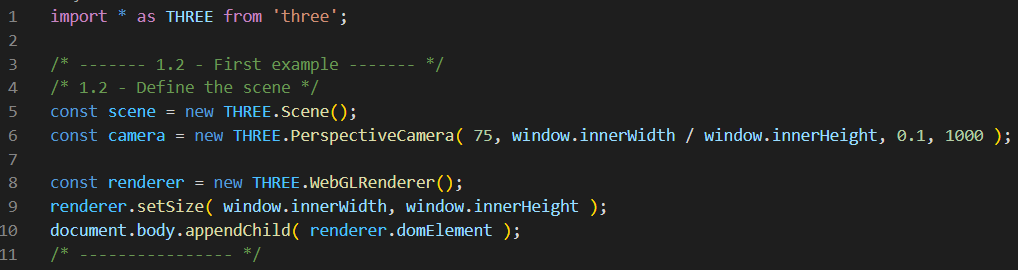
\includegraphics[width = \textwidth]{figs/ex12_1.png}
        \caption{Code for definition of the scene, camera and renderer of 1.2 - First example.}
        \label{figs:ex12_1}
\end{figure}

First is created a scene that works as a container that holds all the objects, lights, and cameras in a 3D environment. Then, it is created a camera that creates a new perspective.\newline
This renderer is used to display the 3D scene using WebGL, which is a JavaScript API for rendering interactive 2D and 3D graphics in compatible web browsers. It is set with the window sizes.\newline
The final line appends the renderer to the html main body element.

%%%%%%%%%%%%%%%%%%%%%%%%%%%%%%%
\subsection{Definition of an object/geometry and camera position}

The code used to make this definitions was the one on Figure \ref{figs:ex12_2}.

\begin{figure}[h!]
    \centering
        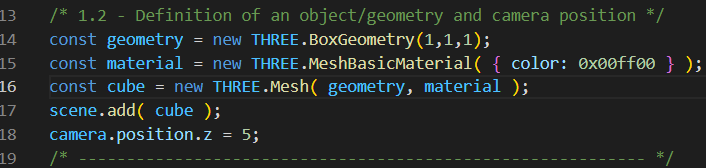
\includegraphics[width = \textwidth]{figs/ex12_2.png}
        \caption{Code for definition of an object/geometry and camera position of 1.2 - First example.}
        \label{figs:ex12_2}
\end{figure}

The where a new instance of THREE.BoxGeometry is created represents a cube or rectangular box in three-dimensional space. The parameters 1, 1, 1 define the width, height, and depth of the box, respectively. The instance of THREE.MeshBasicMaterial is a simple material that is not affected by lights. The cube variable holds a 3D cube by putting a material on a geometry.\newline
The add function adds the created cube mesh to the scene and the camera one sets the position of the camera along the z-axis to 5 units.

%%%%%%%%%%%%%%%%%%%%%%%%%%%%%%%
\subsection{Scene rendering \& animation}

The code used to make this definitions was the one on Figure \ref{figs:ex12_3}.

\begin{figure}[h!]
    \centering
        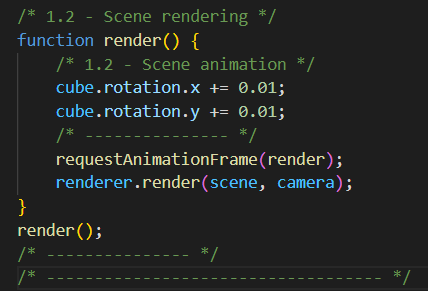
\includegraphics[width = \textwidth]{figs/ex12_3.png}
        \caption{Code for scene rendering \& animation of 1.2 - First example.}
        \label{figs:ex12_3}
\end{figure}

Here, it is created a function that make an animation by updating the rotation of the cube.\par

Next, it used a method that tells the browser that we wish to perform an animation and requests that the browser to call a specified function to update an animation; the last line of the function is responsible for rendering the 3D scene.

%%%%%%%%%%%%%%%%%%%%%%%%%%%%%%%
\clearpage
\subsection{Results}

In Figure \ref{figs:ex12_result} it is represented on frame of the animation obtained.

\begin{figure}[h!]
    \centering
        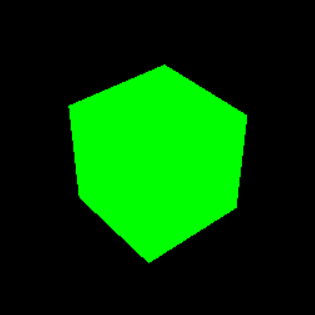
\includegraphics[width = \textwidth]{figs/ex12_result.png}
        \caption{Result of 1.2 - First example.}
        \label{figs:ex12_result}
\end{figure}

%%%%%%%%%%%%%%%%%%%%%%%%%%%%%%%%%%%%%%%%%%%%%%%%%%%%%%%%%%
\section*{1.3 - 2D primitives}
\label{ex_13}

In this exercise we were asked to modify the previous example to visualize a black 2D triangle and to create another material so that the triangle is black over a red background without modifying the camera position.\par

To obtain a triangle we needed a new geometry so, we commented the previews one and created a new one as a buffer. Then we defined the three vertex of the triangle. Finally, we assign vertex data to the buffer specifying that the attribute is composed of three values per vertex, corresponding to the (x, y, z) coordinates; Figure \ref{figs:ex13_1}.

\begin{figure}[h!]
    \centering
        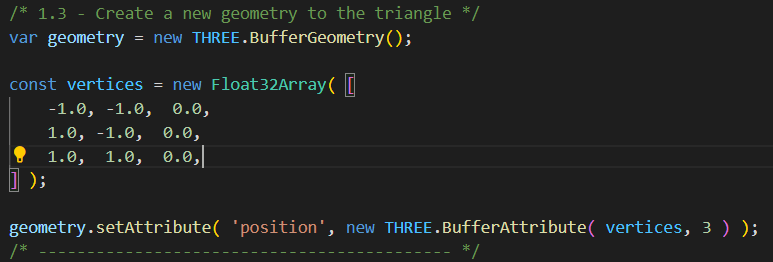
\includegraphics[width = \textwidth]{figs/ex13_1.png}
        \caption{Code for the triangle definition of 1.3 - 2D primitives.}
        \label{figs:ex13_1}
\end{figure}

For the new color scheme, we define a new material with a wanted color and, to define the color of the background, we have used the ".setClearColor" function; Figure \ref{figs:ex13_2}.

\begin{figure}[h!]
    \centering
        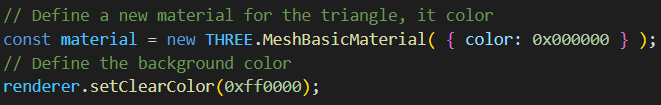
\includegraphics[width = \textwidth]{figs/ex13_2.png}
        \caption{Code for the triangle color definition of 1.3 - 2D primitives.}
        \label{figs:ex13_2}
\end{figure}

The result, a frame of the animation, is represented in Figure \ref{figs:ex13_resutl}.

\begin{figure}[h!]
    \centering
        
\includegraphics[width = \textwidth]{figs/ex13_result.png}
        \caption{Result of 1.3 - 2D primitives.}
        \label{figs:ex13_resutl}
\end{figure}

%%%%%%%%%%%%%%%%%%%%%%%%%%%%%%%%%%%%%%%%%%%%%%%%%%%%%%%%%%
\section*{1.4 - Addition of color}
\label{ex_14}

In this exercise we were asked to represent multiple objects as the ones in Figure \ref{figs:ex14_exemplo}.

\begin{figure}[h!]
    \centering
        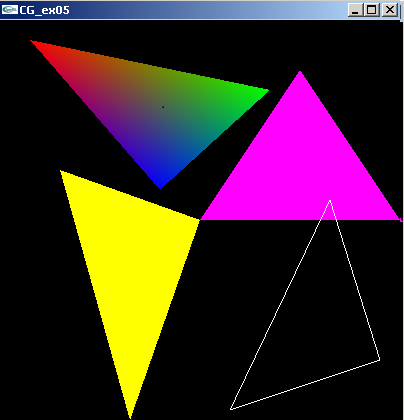
\includegraphics[width = \textwidth]{figs/ex14_exemplo.png}
        \caption{Example of 1.4 - Addition of color.}
        \label{figs:ex14_exemplo}
\end{figure}

\noindent
As it possible to notice, there are four triangles, three full painted and one with only the frame. In order to get this result, we decided to create 4 models, 1 for each triangle.\par

It was created a geometry buffer for each model as well as a color map for the triangle with multiple colors. It is necessary to associate a color to each vertex. The definition of the colors it is represented in Figure \ref{figs:ex14_1}. It is important to mention that the vertices of each triangle follows the same syntax are the previews, like the one on section \ref{ex_13}, and similar to the colors.

\begin{figure}[h!]
    \centering
        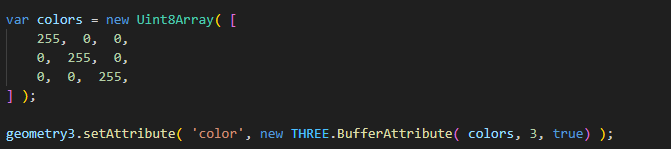
\includegraphics[width = \textwidth]{figs/ex14_1.png}
        \caption{Code for color definition of 1.4 - Addition of color.}
        \label{figs:ex14_1}
\end{figure}

Some triangles were not seen because the face of the triangle with color was not the face that the camera was seeing. One way to fix this problem was using the "THREE.DoubleSide", which made both faces of the triangle use the color defined. The way we fixed it was by changing the order of the vertices, meaning that the triangle with be drawn in a different order and the face with color would be the face towards the camera. 

For the frame triangle an extra parameter was implemented, the "wireframe:true". The code is represented in Figure \ref{figs:ex14_2}.\par

This time, the animation was removed.

\begin{figure}[h!]
    \centering
        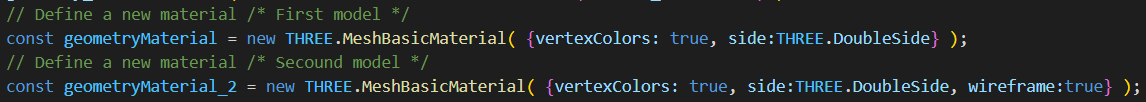
\includegraphics[ width =\textwidth]{figs/ex14_2.png}
        \caption{Code for material definition of 1.4 - Addition of color.}
        \label{figs:ex14_2}
\end{figure}

The result obtained is represent on Figure \ref{figs:ex14_result}. As it is possible to notice, our solution agrees with the example one, on Figure \ref{figs:ex14_exemplo}.

\begin{figure}[h!]
    \centering
        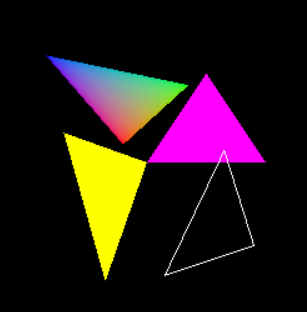
\includegraphics[height = 0.3\textheight, width = 0.8\textwidth]{figs/ex14_result.png}
        \caption{Result of 1.4 - Addition of color.}
        \label{figs:ex14_result}
\end{figure}

%%%%%%%%%%%%%%%%%%%%%%%%%%%%%%%%%%%%%%%%%%%%%%%%%%%%%%%%%%
\section*{1.5 - View-port Update}
\label{ex_15}

For the penultimate we were challenged to change the dimensions of the browser window. We noticed that the visualization window is not update when the browser window size changes. In order to solve this problem, we were told to create a new function to be called when the browser window size is updated.\par

The function created as access to the the window size so it is possible to update size of the renderer accordingly. It also needs to modify the aspect camera ratio as well and update this change. The code to obtain this function is represented in Figure \ref{figs:ex15_1}.

\begin{figure}[h!]
    \centering
        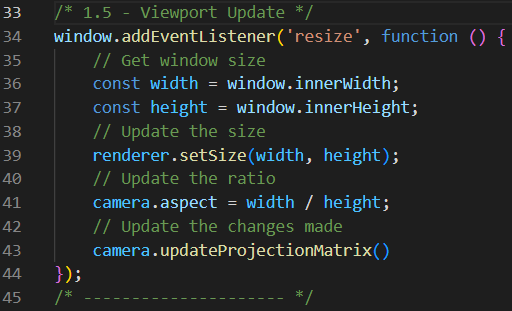
\includegraphics[ width = \textwidth]{figs/ex15_1.png}
        \caption{Code for the function of 1.5 - View-port Update.}
        \label{figs:ex15_1}
\end{figure}

The result is illustrated on Figure \ref{figs:ex15_result} and, as it is possible to see, with the function developed on Figure \ref{figs:ex15_1}, the left cube remains on the window. On the right, without the window update, the cube stays in the same position and if the window is re-sized. the cube despairs.

\begin{figure}[h!]
    \centering
        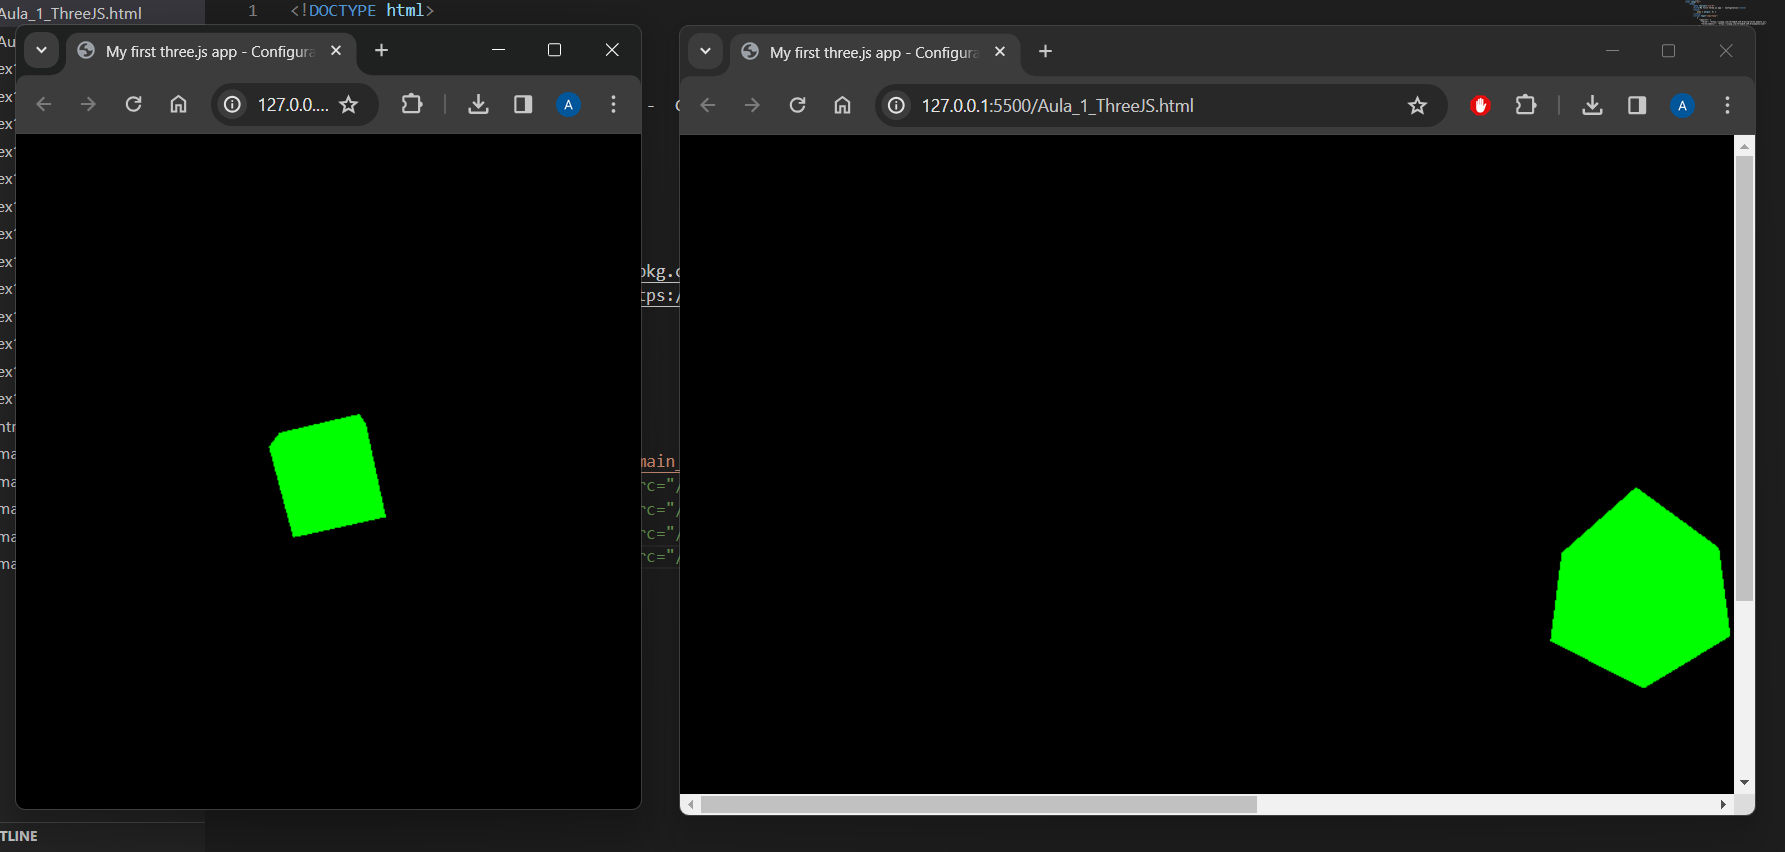
\includegraphics[ width = \textwidth]{figs/ex15_result.png}
        \caption{Result of 1.5 - View-port Update.}
        \label{figs:ex15_result}
\end{figure}

%%%%%%%%%%%%%%%%%%%%%%%%%%%%%%%%%%%%%%%%%%%%%%%%%%%%%%%%%%
\section*{1.6 - Other primitives}
\label{ex_16}

For the final exercise we were asked to modify the first example to show the cube in wire-frame and investigate other available geometries and visualize at least 4 other geometries in the same scene changing some of their default parameters.\par

We have explored the geometries presented on Figure \ref{figs:ex16_result}.

\begin{figure}[h!]
    \centering
        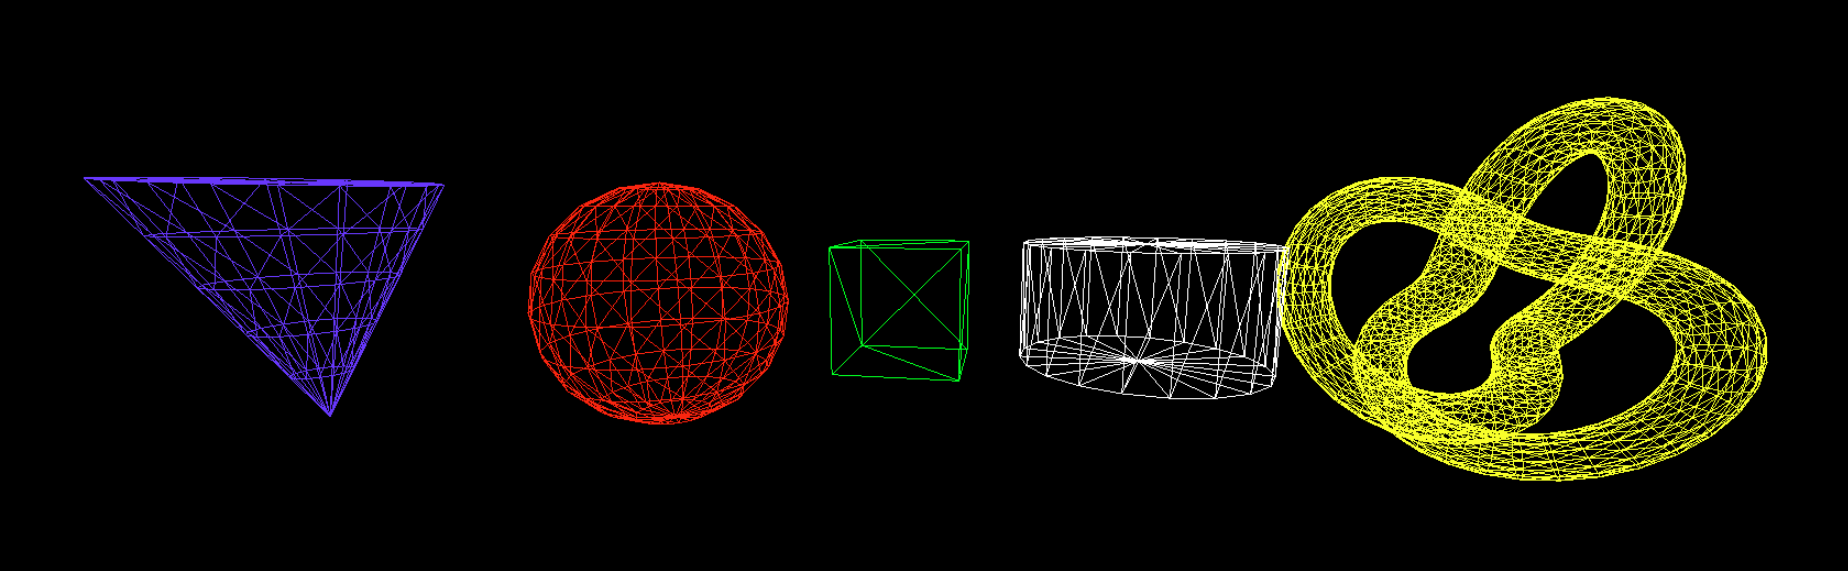
\includegraphics[ width = \textwidth]{figs/ex16_result.png}
        \caption{Result of 1.6 - Other primitives.}
        \label{figs:ex16_result}
\end{figure}

To achieve this geometries we follow the same logic as the Exercise 1.2 - First example. This time we've also explore a sphere, a cone, a cylinder, and a torus knot geometries.\newline
To get that shapes, we have used the code on Figure \ref{figs:ex16_1}.

\begin{figure}[h!]
    \centering
        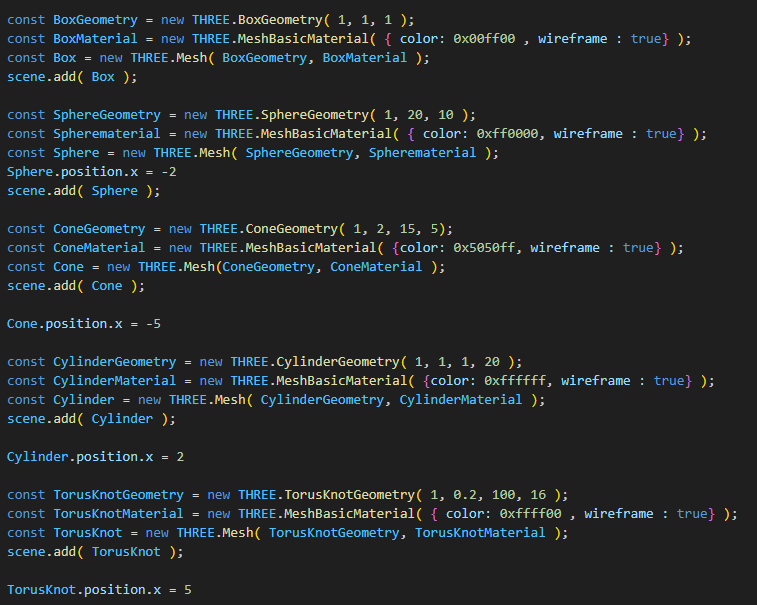
\includegraphics[ width = \textwidth]{figs/ex16_1.png}
        \caption{Code for 1.6 - Other primitives.}
        \label{figs:ex16_1}
\end{figure}

\noindent
As it possible to see, instead of "THREE.BoxGeometry", it was used "THREE.SphereGeometry", "THREE.ConeGeometry",  "THREE.CylinderGeometry" and "THREE.TorusKnotGeometry". The animation is performed equal to each object.

%%%%%%%%%%%%%%%%%%%%%%%%%%%%%%%%%%%%%%%%%%%%%%%%%%%%%%%%%%
\section*{Conclusion}
\label{Concl}

To sum up, we consider that the Lesson 1 -  three.js Introduction was concluded with success because all exercises were completed successfully and presented results were as expected.

%%%%%%%%%%%%%%%%%%%%%%%%%%%%%%%%%%%%%%%%%%%%%%%%%%%%%%%%%%

\end{document}

